\part{Synthesis}
	\chapter{Introduction}
	Now that the relevant product fields are understood to a sufficient degree and the product's needs have been established we can begin to plan out how we will achieve the project's objectives. First we will established the methological approach that will structure the product's development. Then, for each of the core product requirements we will look at a high level design overview of how the requirement will be met, the actual implementation of this design, and testing to evaluate how well this requirement has been satisfied by this implementation.
	
	\chapter{Methological Approach}
	The project employed a prototyping methodology for development. First, we must perform an investigation into the system requirements, which was performed in the analysis with a list of specific core requirements being outlined in the conclusion. Following this the first prototype is built, which will resemble an incredibly basic scaled down version of how the final system should ideally look. This prototype is then thoroughly evaluated, with potential changes that would bring the prototype closer to the final system being figured out. Finally, these changes are then implemented and the prototype is evaluated once again. This is repeated until the product has reached its ultimate goals.
	\begin{figure}[h]
		\centering
		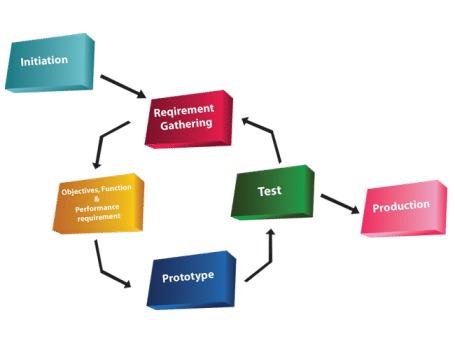
\includegraphics[width=.8\linewidth]{SYNTHESIS/prototypingdiagram.png}
		\caption{Prototyping Methodology}
		\label{fig:prototypingdiagram}
	\end{figure}
	
	This methodology was employed partially due to the hardware nature of the product. Key features of the robot hinged on aspects like movement and observation being possible, so it was important to get a prototype that has this basic functionality up and working and quickly as possible. The prototyping approach allowed a pure focus on getting these functions working, and once they were the robot could be improved iteratively.
	
		\subsection{Initial Prototype}
		As previously stated, this methodology involves an initial prototype that all future prototypes will be an iteration of. The initial prototype of the project will involve the basic, primary construction of the robot. This will first involve the basic chassis assembly followed by attempting to connect relevant components to eachother. Once this is done, we'll hopefully have an incredibly crude robot that won't be capable of anything, but should hopefully serve as a solid foundation for future development toward the project goals.
		
		A similar approach will be followed for processing the map data. It won't be developed simultaneously at first as the robot needs to be capable of storing observational data from the LIDAR before the program can actually do anything, however it will start to be put together once the robot crosses this developmental threshold.
	
	\chapter{Design}
		\section{Introduction}
		Before implementation of the specific project aims can be implemented, we first need the initial prototype that we can begin iteratively improving. Therefore, it's logical to design the initial robotic prototype first. What follows is an overview of how the initial robot prototype will be designed, followed by a breakdown of each of the individual project aims will be met.
	
		\section{Initial Prototype}
		Here will be the design for the base product that will serve as a foundation for all subsequent the development. The aim here is to have a skeleton project that can be filled in with functionality and built on to meet the project objectives.
		
			\subsection{Hardware}
				\subsubsection{Chassis}
				First off will be the basic assembly of the three wheeled omnidirectional chassis. The chassis is comprised of two triangular metal plates, which will be joined together by screwing metal rods into pre drilled holes on each of the platforms. The lower platform is where the motors and mounting points for the omnidirectional wheels are found, so once the plates have been connected the wheels will be pushed onto these mounting points and locked into place. Fig \ref{fig:chassisassembly} shows the assembly document that came with the chassis.
				\begin{figure}[h]
					\centering
					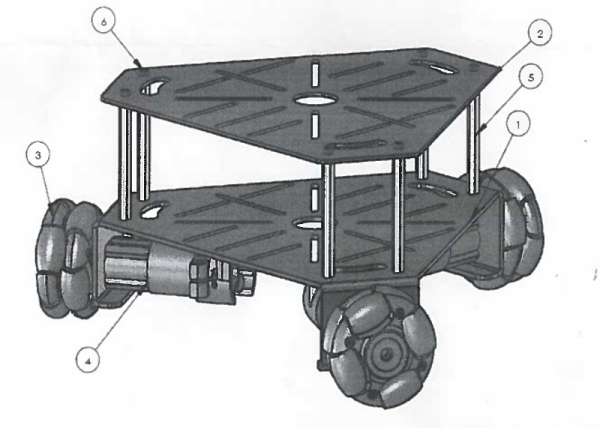
\includegraphics[width=.9\linewidth]{SYNTHESIS/chassisassembly.png}
					\caption{Chassis assembly guide}
					\label{fig:chassisassembly}
				\end{figure}
				
				Now it's time for the microcontroller setup. The microcontroller used in this project is the FRDM-K64F, chosen for its free availability from the University loan office, small form factor and compatibility with the Micro C Operating System which is being employed for the robot's core program. To control the robot we'll also need a motor driver. The dfRobot Quad Motor Driver Shield is being employed for this project, it can be obtained from Amazon for around \pounds{13}. It was chosen for this relatively low cost, the easily available documentation and the fact that it can easily plug into the FRDM-K64F, the microcontroller of choice for this project. This shield will be lined up to the appropriate pins on the K64F and plugged in, in preperation for using the microcontroller to drive the motors. 
				
				The assembly shouldn't be overly complex, no soldering should be needed to connect components so it should be mostly a case of fitting things together.
				% explain LIDAR later.... :(
			\subsection{Software}
				\subsubsection{Robot Program}
				As previously mentioned in the analysis, the robot's program will be composed of a Micro C OS. Once further design has been discussed and a good idea of how the program should be structured has been understood, it would be prudent to create a skeleton OS with some basic tasks that simply print to ensure first that software can be properly deployed onto the microcontroller, and secondly to speed up development by allowing individual parts of the OS to be developed straight away.
				
			\subsection{Power}
			The hardware components that will need powering are the three motors used to drive the omnidirectional wheels, the microcontroller, and the LIDAR sensor. Table \ref{table:1} has a run down of these hardware components, the voltages, and the milliamp consumption that they have.
				
			\begin{table}[h]
				\centering
				\begin{tabular}{|| l | l | l ||} 
					\hline
					Component & Voltage & Milliamp \\ [0.5ex] 
					\hline
					3x DC Coreless Motor  & 12V & Up to 1400 mA  \\ 
					FRDM-K64F  & 5 to 9V &  50 mA \\
					RPLIDAR  & 5 to 10V & Up to 1050 mA\\
					\hline
				\end{tabular}
				\caption{Components and respective voltages}
				\label{table:1}
			\end{table}
			
			To save on cost and complexity, it would be ideal to only use a single battery for the robot's power source. A single power source will be used for the robot, a battery holder containing 8 1.5V batteries will give us the 12V we need for the motors. Then, a step down voltage regular will be used to lower the voltage required for the other components. A 7v and two 5v currents will be needed to supply power to the microcontroller and the LIDAR respectively.
			% !!!!!!!!!!!!!!!!!!!!!!!COME BACK TO THIS!!!!!!!!!!!!!!!!
				
			Generally cheaper alkaline batteries have about 1800 to 2800 mAh (milliamp hours) in them, so an 8 pack of these will give us about half an hour's worth of operation before the robot starts to suffer due to low power. This is a worst case scenario assuming a constant high power draw, but this should be sufficient for the purposes of prototyping and demonstration. 
			
			\subsection{Software}
			The software for the actual robot will be written in C++, compiled and deployed onto the microcontroller with the mbed SDK. At its foundation, it will be a Micro C OS with a series of configured tasks to perform various aspects of the robot's functionality. As would be expected, these tasks will come with their own memory tasks and will be designated with appropriate priorities. 
			
			The plan is for there to be three separate tasks. One task will deal with the robot's movement, one task will deal with taking data from the LIDAR and the final task will deal with actually writing this scan data to the connected Micro SD-Card. To control the program flow semaphores will be employed. For the initial prototype, these three tasks will be initialized and simply print messages to the console so a program such as minicom can see them running. This will allow assurance that the tasks are running in a logical order.
		
		\section{Designing for Requirements}
		Once this incredibly basic initial prototype is in place, we can begin to move toward truly fulfilling the project requirements. What follows is an overview of how each of the different project requirements will be met, with appropriate explanations toward the hardware and software employed.
		
			\subsection{Movement}
			The first of the three product aims outlined in the Analysis is that 'the robot must be capable of movement'.
				\subsubsection{Hardware}
				The dfRobot Quad Motor shield is being used to help control the motors. Fig \ref{fig:shield} shows an overview of the shield.
				\begin{figure}[h]
					\centering
					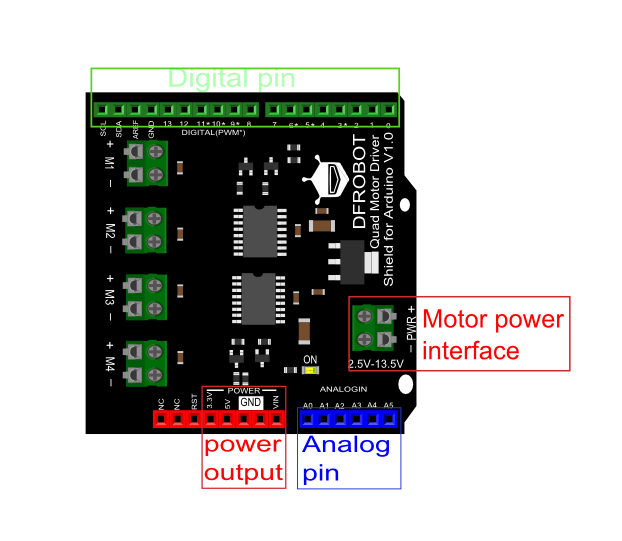
\includegraphics[width=.7\linewidth]{SYNTHESIS/QuadMotorDriverShield.png}
					\caption{Example shield setup}
					\label{fig:shield}
				\end{figure}
			
				The motor power interface is how the shield will actually recieve its power from the battery. The power and ground cables from each of the chassis motors will be plugged into the appropriate motor pins that can be seen on the left of the shield figure. Fig \ref{fig:shieldsetup} from the shield's documentation shows an example of this setup with four motors.
				
				\begin{figure}[h]
					\centering
					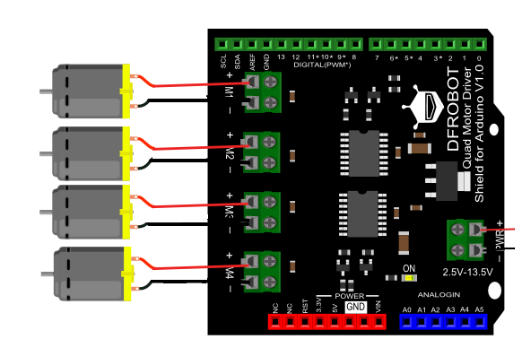
\includegraphics[width=.7\linewidth]{SYNTHESIS/shield_connection.png}
					\caption{Example shield setup}
					\label{fig:shieldsetup}
				\end{figure}
				
				Each of the motors power and ground cables will connect to the appropriate pins on the shield. The motors can be manipulated once they receive power in this fashion. The shield is able to affect the electricity being sent to the motors by changing its polarity and by using pulse width modularity. By changing the pin to HIGH or LOW, we can affect the direction that the motor spins in (forward or backwards) and pulse width modulation allows us to affect the speed of the motor.
				
				\subsubsection{Software}
				For each motor on the shield, there are two associated pins. The first of these pins controls the motors direction (forward or backward). The second of the pins controls the motor speed,  achieved using pulse width modulation. To manipulate the motors these pins will need to be declared as variable within the robot's software and assigned different values based on what we are trying to do. The directional pins are either HIGH or LOW, so they will be declared as digital pins that are assigned a binary value. For the speed pins, mbed features a PwmOut interface with a .write() method that can be used to assign a duty cycle value to the variable. This is perfect for what we need.
				%talk about pin lineup here and declaration
				% COME BACK TO THIS, TRIGONOMICAL NAVIGATION!
				
			\subsection{Observation}
			The second of the three product aims outlined in the Analysis is that 'the robot must be capable of observation'.
				\subsubsection{Hardware}
				Only one range finder is being used to gather the observation data, the RPLIDAR A1M8 LIDAR sensor. The sensor is composed of a platform with a motor system that spins the range scanner as it takes readings, as well as some pins that can be used for communication. Fig \ref{fig:rplidarconfig} illustrates these components.
				
				\begin{figure}[h]
					\centering
					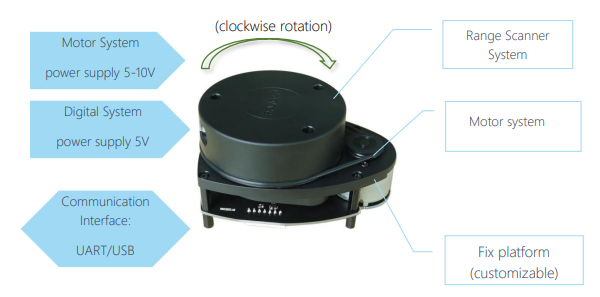
\includegraphics[width=.9\linewidth]{SYNTHESIS/rplidar_configuration.png}
					\caption{LIDAR Underside}
					\label{fig:rplidarconfig}
				\end{figure}
			
				There are seven pins on the underside of the LIDAR sensor, shown in fig \ref{fig:lidarunderside}. These pins need to be connected to the appropriate microcontroller ports if the LIDAR is to work. 
				\begin{figure}[h]
					\centering
					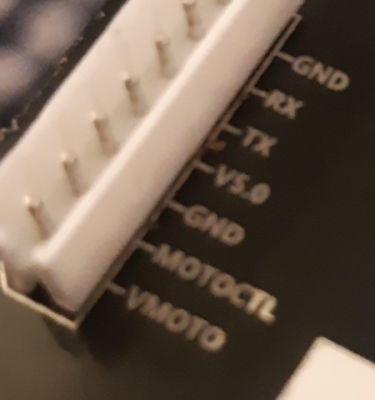
\includegraphics[width=.4\linewidth]{SYNTHESIS/lidarunderside.png}
					\caption{LIDAR Underside}
					\label{fig:lidarunderside}
				\end{figure}
				
				The GND pins are simple ground pins, they will need to be connected to ground pins on the microcontroller. The RX and TX pins (Recieve and Transmit respectively) are serial pins that will be used for communication with the microcontroller. These LIDAR pins will be linked to their opposite counterparts on the microcontroller (LIDAR RX to Microcontroller TX and vice versa). The V5.0 and VMOTO are simple power pins, they will powered via a stepped down 5V current taken from the voltage regulators. This is how the LIDAR sensor will retrieve power. The MOTOCTL pin is the motor control pin that listens for a signal indicating that a connected device is ready to recieve data. The signal is either high (ready) or low (not ready). To make use of this pin, a generic GPIO pin from the microcontroller will be configured within the microcontroller's software and set to 1 (high) when the robot needs to begin taking scan data.
				
				\subsubsection{Software}
				SLAMTEC have a document detailing the LIDAR protocol. This details the specifics behind how to communicate with the LIDAR. LIDAR communication is primarily achieved through the exchange of data packets. As a basic example, in order to obtain scan measurements the host system first needs to send data packets corresponding to the begin scan command. Once the LIDAR has recieved and processed this, it should begin sending back observational data. 
				
				The format of the requests that need to be sent is documented in the LIDAR's protocol documentation\citep{rplidarprotocol}. To implement this, it would be a good idea to create a data structure in the microcontroller's C++ program with fields listed in the protocol (start flag, command, etc) and then put this field into the serial connection. A similar data structure could be populated with what is recieved from the serial channel to make it easy to process the data.
				
				SLAMTEC provide an SDK for the LIDAR sensor however, which comes in the form of header files which will automatically implement this functionality. Table \ref{table:sdkbreakdown} has a manifest of the SDK and the functionality that it provides.
				
				\begin{table}[h!]
					\centering
					\begin{tabular}{|| l | l ||} 
						\hline
						File & Purpose \\ [0.5ex] 
						\hline
						rplidar.h  & Parent file for subsequent header files  \\ 
						rplidar\textunderscore driver.h  & Provides RPLidarDriver class for  interfacing with sensor   \\
						rplidar\textunderscore  protocol.h  & Defines structs and constants for the LIDAR protocol  \\
						rplidar\textunderscore  cmd.h & Defines request/answer structs for LIDAR protocol  \\ 
						rptypes.h & Platform independent structs and constants  \\ [1ex] 
						\hline
					\end{tabular}
					\caption{RPLIDAR SDK files}
					\label{table:sdkbreakdown}
				\end{table}
				
				Essentially, the C++ program running on the microcontroller would need to create an RPLidarDriver variable which would be used to represent the connected LIDAR sensor. Once this is achieved the premade methods that implement the protocol functionality could be ran to achieve control over the LIDAR.
				
			\subsection{Processing Observational Data}
			The last of the three project objectives is that 'the observational data must be processed into a map'.
				\subsubsection{Hardware}
				Once the robot is receiving data from the LIDAR sensor, it needs to be transferred to an external program where the CSM software can be ran to generate a map from it. Based on the results of the previously conducted investigation into what would be the most suitable way to store observational data, a Micro SD-Card will be used. The FRDM-K64F has a Micro SD-Card socket attached to it, and the microcontroller will save the observational data to this card so that after a session of moving and scanning it can be plugged into a machine where it is able to be processed. The University's loans office can provide an 8GB card as well as an adapter allowing it to be plugged into a PC's USB slot, so this approach won't incur any extra cost. The saved data will only be angle and distance measurement pairs, so the card's (relatively) small size won't pose any memory issues. 
				
				\subsubsection{Software}
				First, the microcontroller must save this data to the connected Micro SD-Card. Mbed has a library called SDFileSystem used for interaction with connected SD cards. Using this library, a simple text file will be created on the Micro SD-Card and angle/distance measurements obtained from the LIDAR sensor will be written to it. This file will be written to the SD-Card after all movement and scanning has been done to keep the program simple. The FRDM-K64F features 256kB of RAM, and a C float is around 4 bytes. If we quite generously assume 156kB will be taken up by task stacks and other program necessities, that still leaves around 100kB of free RAM. In 100000 bytes, we can still store 25000 floats in RAM. Given that each returned scan will probably have two floats (an angle and a distance) we can store at least 12500 readings which is a good few seconds of LIDAR data.
				
				Once readings have been written to the SD-Card, it will be removed and plugged into a USB adapter so it can be plugged into a computer. For ease of use, a GUI program will be used to automate the rest of the functionality. To design the GUI, a Python library called Tkinter will be used. It offers all the widgets that will need to be used to make a basic GUI such as frames, buttons and labels and its support of most (if not all) operating systems will allow it to be easily used. The GUI's job then is to create an appropriate input for CSM and to use it to generate a map from the readings. CSM takes in readings in the form of either a json or a carmen log. Of the two, json will be used due to its familiarity and much more easily accessible documentation around the internet. To invoke the CSM software itself via the program, Python features a subprocess module which allows for Python programs to spawn simple subprocesses and retrieve information they return. Once the software has processed a map from the readings, it will be output onto the screen so that the user can view it.
		\newpage
		\section{Pseudo Code}
		To help illustrate the system's overall design some pseudo code has been made. To prevent it from being overcomplicated some aspects such as the declaration of task priorities or memory stacks have been omitted, the pseudo code's purpose is not to show each and every aspect of what needs to be implemented but rather to serve as a structural guide during the implementation.
		%PSEUDO CODE HERE, COPY FINAL ROBOT CODE
		\begin{lstlisting}
			FileSystemDeclaration
			LIDARSerialConnectionDeclaration		
			
			scanningSemaphore
			writingSemaphore
			
			movementTask() {
				acquireSemaphores
				move
				releaseScanSemaphore
				pendScanSemaphore
				releaseWritingSemaphore
				pendWritingSemaphore
			}
			
			scanTask() {
				pendScanSemaphore
				scan
				releaseScanSemaphore
			}
			
			writeTask() {
				pendWritingSemaphore
				write
				releaseWritingSemaphore
			}
		\end{lstlisting}
		
	\chapter{Implementation}
		\section{Introduction}
		This chapter will describe the actual creation of the product. The implementation of relevant software and hardware features for the different product components will be discussed, as well as unforeseen problems that were encountered.
		
		\section{Initial Setup}
		Before work can begin implementing any specific functionality for the robot, some preliminary hardware assembly and software setup had to be carried out.
			
			\subsection{Hardware}
			First of all the physical chassis had to be assembled. The only available documentation was fig \ref{fig:chassisassembly}, a labeled picture of an already assembled chassis which wasn't terribly useful. Luckily the construction was relatively straight forward, and only took around thirty minutes. Once the structure was built, the wheels where pushed onto the motors where they clicked on. The Quad Motor Shield was then installed onto the K64F microcontroller without any problems.
				
			\subsection{Software}
			To speed up later development a basic Micro C OS was created and deployed onto the microcontroller. This OS resembled the pseudo code and was composed of skeleton tasks that simply printed their task name to the console when they ran. Semaphores were initialized and combined with the print messages the basic program flow could be figured out.

		\section{Implementing Requirements}
			\subsection{Movement}
				\subsubsection{Hardware}
				First the dfRobot Quad Motor shield was fitted onto the K64F microcontroller and placed in the lower level of the robot. Each of the three wheel motors had a ground and a power cable attached to them, these were all fed through the hole in the centre of the lower plate and connected to the appropriate ports on the motor shield. In the interest of keeping the components tidy, the power and ground cables were fastened to the lower plate with zip ties.
				
				Each pair of power and ground ports are labelled with a number on the shield (e.g M1, M2 etc). From hereonn in, the motors will be referred to with these same numbers. Fig \ref{fig:robotwheels} shows the position and names of each of the wheels on the robot.
				% FIG HERE
			

				
				
				At this point it was time to power the motors by connecting the 12V battery pack to the motor shield. Initially it was planned that this would be achieved from a breadboard, as the breadboard would allow the use of voltage regulators to supply lower voltages to the other components. A problem was encountered here though in the way of space. The microcontroller, motor power cables and battery pack alone already cluttered nearly all of the lower level of the robot. The additional of a breadboard with voltage regulators and additional wiring would be an incredibly difficult fit with wires potentially breaking or coming loose, and there was still the matter later on of connecting the LIDAR properly. This resulted in two decisions being made. The first was that the LIDAR would simply recieve power from the microcontroller. The second decision was that the microcontroller would receive its own battery. The K64F features a VIN pin for power that takes between 5V and 9V, so a 6V battery pack was obtained. The power cable was connected to the VIN, and the ground cable shared a ground port with the motor's battery pack.
				
				\subsubsection{Software}
				Each of the three motors were now connected to two pins on the Quad Motor Shield. One pin affected direction, the other affected the speed. Direction was a simple case of polarity. Depending on the motor, HIGH or LOW dictated whether the motor span forwards or backwards. These pins could be declared as DigitalOut variables, and assigned either a 1 or a 0 depending on what was needed.  The pins that affected speed did so via pulse width modulation, so these could be declared as PwmOut variables and floats could be assigned to them to affect their duty cycle. The motor driver's documentation has a table stating which of the pins on the shield corresponded to which motors, so whichever K64F pin was connected to the relevant shield pin was used for the variables.
				
				% state specifically which pin for each motor or is that too granular?
				\begin{lstlisting}
				DigitalOut  M1_DIR(D4);
				PwmOut      M1_SPD(D3);
				
				DigitalOut  M2_DIR(D12);
				PwmOut      M2_SPD(D11);
				
				DigitalOut  M3_DIR(D8);
				PwmOut M3_SPD(D5);
				\end{lstlisting}
				
				Simple movement could be achieved just by configuring different motors to spin in different directions initially. Functions were made that allowed the robot to drive in four basic directions. One such function can be seen below.
				\begin{lstlisting}
				static void goForward() {
					pc.printf("goForward");
					M2_DIR = 1;
					M3_DIR = 1;
				
					M1_SPD = 0;
					M2_SPD = 0.5f;
					M3_SPD = 0.5f;
				}
				\end{lstlisting}
				
				This for example set Motor 2 to spin clockwise and Motor 3 to spin counter-clockwise. Both of these wheels therefore moved in the direction of the first motor, and the small rollers on the wheel allowed the robot to frictionlessly slide in this direction.
				
				
			\subsection{Observation}
			Implementation of the robot's ability to take observations about its environment first involved a hardware configuration. The LIDAR sensor needed to be connected to the microcontroller so that it could draw power from the battery, as well as communicate with the microcontroller allowing it to receive commands and send observational data. Once the hardware connection was established, software on the microcontroller had to be capable of operating the LIDAR sensor and recieving its observations.
				\subsubsection{Hardware}
				As previously discussed, the seven pins on the underside of the LIDAR sensor need to be correctly connected up to the appropriate microcontroller pins if the sensor is to be used.
				
				Table \ref{table:4} gives an overview of which LIDAR pins needed to be connected to which microcontroller pins.
				
				\begin{table}[h!]
					\centering
					\begin{tabular}{|| l | l | l ||} 
						\hline
						LIDAR Pin & K64F Pin & Pin Purpose \\ [0.5ex] 
						\hline
						GND  & GND & Ground  \\ 
						RX  & TX  & Serial Communication \\
						TX  & RX & Serial Communication \\
						V5.0 & 5v & LIDAR Core Power \\ 
						GND & GND & Ground \\ 
						MOTOCTL & D7 & DTR (Data Terminal Ready) \\ 
						VMOTO & 3v3 & LIDAR Motor Power \\ [1ex] 
						\hline
					\end{tabular}
					\caption{LIDAR Microcontroller pin setup}
					\label{table:3}
				\end{table}
			
				Due to the dfRobot Quad Motor shield being plugged into the K64F microcontroller, these LIDAR pins need to be connected to ports on the robot shield that are plugged into the appropriate microcontroller pins. Essentially, we look at what port needs to be used on the underlying microcontroller, then plug it into the motor shield port that is sitting on top of it. The LIDAR pins and shield ports were connected using simple male to female connector wires.
				
				With regards to power, it was previously mentioned in the movement implementation that due to spacial constraints the LIDAR would recieve power from the microcontroller. The microcontroller features two pins that can supply a voltage, a 5V pin and a 3V3 pin. Both pins would ideally recieve 5V, but to save room and ensure a simpler robot the scanner motor was connected to the lower voltage pin. It was decided that the scanner motor should recieve the lower voltage because it only appeared to make the scanner move a bit slower, whereas there was a concern that supplying the actual LIDAR core with a lower voltage might result in problems performing the actual scanning. 
				
				Once this was done, the LIDAR was able to function mechanically.
				
				\subsubsection{Software}
				Following the hardware setup the microcontroller needs to actually communicate with the LIDAR sensor so that it can send commands, as well as receive observational data. 
				
				To first of all ensure the LIDAR is ready to communicate, the previously discussed MOTOCTL pin on the LIDAR needs to be recieving a HIGH signal so that it knows the microcontroller is ready to begin recieving data. The K64F features numerous GPIO pins that can be easily configured for usage in situations like this. One such pin (D7) was simply declared as a basic DigitalOut allowing the microcontroller to manipulate the pin's polarity.
				
				% too granular?
				\begin{lstlisting}
				DigitalOut dtr(D7);
				\end{lstlisting}
				
				When we want the sensor to output data this pin can be set to HIGH...
				\begin{lstlisting}
				dtr = 1;
				\end{lstlisting}
				
				...or when we want it to stop, we can set it to LOW.
				\begin{lstlisting}
				dtr = 0;
				\end{lstlisting}
				
				Once this was done and the DTR pin was set to HIGH, the LIDAR began spinning. The microcontroller didn't instantly begin recieving data however, as simply connecting the LIDAR and microcontroller serial pins are not enough for communication. In order to interact with the serial channel it needs to be declared in the robot's core program as an appropriate variable. There exists a library for arm MBED microcontroller called BufferedSerial which can be used for this. The original Serial library that it is based on allows for serial communication, with BufferedSerial simply adding a buffer to this. The core functionality remains the same however.
				
				First the pins being used for serial communication need to be declared as a BufferedSerial variable, with BufferedSerial taking the TX and RX pin (in that order) of the microcontroller. 
				\begin{lstlisting}
				BufferedSerial lidar_device(D1, D0);
				\end{lstlisting}
				
				As previously discussed in the Design, SLAMTEC has an SDK that automates most of the LIDAR functionality. The appropriate files were added to the project and made able to be used by the core program with a simple include statement at the top of the main.cpp file.
				\begin{lstlisting}
				RPLidar lidar;
				\end{lstlisting}
				
				Following this a base lidar variable can be declared from the RPLidar class the SDK adds.
				\begin{lstlisting}
				RPLidar lidar;
				\end{lstlisting}
				
				Once this variable has been declared, in the program's main method the DTR is set to 0 to ensure that the LIDAR won't start scanning and outputting data when we don't need it to. The LIDAR variable is then connected to the relevant serial variable (the previously declared BufferedSerial) and the start scan command is issued. Despite receiving the command to start scanning the LIDAR won't begin until the DTR gives it the go ahead, but by configuring this as soon as the program begins it's a lot easier to stop and start the LIDAR data output.
				\begin{lstlisting}
				dtr = 0;
				lidar.begin(lidar_device);
				lidar.startScan();
				\end{lstlisting}
				
				From here, two different simple one-line methods are used to start and stop the lidar.
				\begin{lstlisting}
				static void beginScanning() {
					dtr = 1;
				}
				
				static void stopScanning() {
					dtr = 0;
				}
				\end{lstlisting}
				These methods allow for quick and easy configuring of the DTR pin.
				
				Now that the LIDAR is configured and can begin sending out data, it's time to start actually storing it within the program. First we need appropriate mediums for the storage of LIDAR data. This entails something to store a LIDAR sample that has just arrived so we can manipulate it to take what we need from it, and also a buffer to store all the total readings collect so that they can later be written to disk. 
				
				In order to store a newly recieving reading, the RPLidar SDK implements a basic struct that can be filled in with a .getCurrentPoint() method. This will be used so that recieved readings can be easily manipulated.
				\begin{lstlisting}
				struct RPLidarMeasurement
				{
					float distance;
					float angle;
					uint8_t quality;
					bool  startBit;
				};
				\end{lstlisting}
				
				Now we need somewhere to store the readings themselves so they can be written to disk later on. We're interested in storing a large number of angle/distance pairs, so a large two dimensional array was used.
				\begin{lstlisting}
				float readingsBuffer[16000][2];
				\end{lstlisting}
				A two dimensional array was used to ensure an understandable format to the array. The array has 16000 spaces, with each space storing two seperate float values (angle and distance respectively). Now the actual method to take LIDAR readings and store them in the buffer needs to be made.
				
				Now that readings can be manipulated and stored, it's time to properly implement the method that stores them to a buffer.
				\begin{lstlisting}
				static void takeReadings() {
					int arraySize = (sizeof(readingsBuffer)/sizeof(float))/2;
					struct RPLidarMeasurement measurement;
					for(int i = 0; i < arraySize; i++) {
						lidar.waitPoint();
						measurement = lidar.getCurrentPoint();
						readingsBuffer[i][0] = measurement.angle;
						readingsBuffer[i][1] = measurement.distance;
					}
				}
				\end{lstlisting}
				The method iterates through the buffer and stores the angle and distance of each reading it receives.
				
				All of these methods can now be incorporated into the scan task.
				\begin{lstlisting}
				static void appTaskScan(void *pdata) {
					uint8_t status;
				
					while(true) {
						OSSemPend(readyToScan, 0, &status);
						pc.printf("Scanning...\n");
						beginScanning();
						takeReadings();
						stopScanning();
						pc.printf("Stopping scan.\n");
						status = OSSemPost(readyToScan);
						OSTimeDlyHMSM(0,0,0,4);
					}
				}
				\end{lstlisting}
				Once the readyToScan semaphore has been released, the scan task acquired it and the LIDAR begins scanning. Then the readings are stored to the buffer so they can be written to the disk later and the LIDAR stops scanning. It then releases the semaphore so that the movement task can begin again.		
				
			\subsection{Processing Observational Data}
			Processing the observational data first involves actually finding a way to take it from the robot. It was determined that the best way to implement this would be via the use of a Micro SD-Card. Once this was done, the data itself needed to be turned into some form of map.
			
				\subsubsection{Hardware}
				The only hardware elements that were needed to implement this functionality were the Micro SD-Card socket on the microcontroller, a Micro-SD card and a USB adapter allowing for a computer to access the files on the SD-Card. The socket was already attached to the microcontroller and no adjustments needed to be made to the hardware for the microcontroller to access it.
				
				\subsubsection{Software}
				In order to access the Micro SD-Card the SDFileSystem library was used, and was incorporated into the program by simplying including the main SDFileSystem header. To use the library, an SDFileSystem variable first needs to be instantiated. This variable takes five parameters, four relevant microcontroller pins and a name. Table \ref{table:sdfilesystempins} describes each of the four pins the SDFileSystem needs, the name of the corresponding microcontroller pin and what the pin actually is.
	
				\begin{table}[h!]
					\centering
					\begin{tabular}{|| l | l | l ||} 
						\hline
						SDFileSystem Parameter & K64F Pin & Pin Purpose \\ [0.5ex] 
						\hline
						MOSI  & PTE3 & Master Out Slave In \\ 
						MISO  & PTE1  & Master In Slave Out \\
						SCLK  & PTE2 & Serial Clock \\
						CS & PTE4 & Chip Select \\ [1ex] 
						\hline
					\end{tabular}
					\caption{SDFileSystem Setup}
					\label{table:sdfilesystempins}
				\end{table}
			
				The code risks being unclear if regular pin names are always used, so the relevant pins were first defined into more understandable names. The SDFileSystem variable was then declared.
				
				\begin{lstlisting}
				#define MOSI		PTE3
				#define MISO		PTE1
				#define	SCLK		PTE2
				#define	CS				PTE4
				
				SDFileSystem sd(MOSI, MISO, SCLK, CS, "sd");
				\end{lstlisting}
				
				With this variable the file system on the Micro SD-Card is able to be accessed. The previously described scan task is what populates the readingsBuffer with data that is needed, so a method is required to iterate through the buffer and write the observational data to the Micro SD-Card.
				
				\begin{lstlisting}
				static void writeReadings() {
					int arraySize = (sizeof(readingsBuffer)/sizeof(float))/2;
				
					// Create the readings file on the Micro SD-Card
					FILE *fp = fopen("/sd/readings.txt", "w");
				
					// Error checking
					if (fp == NULL) {
						pc.printf("Unable to access/create file \n");
					}
				
					// Iterate through the readingsBuffer and write the angle/distance pairs
					for(int i = 0; i < arraySize; i++) {
						fprintf(fp, "%f,%f ", readingsBuffer[i][0], readingsBuffer[i][0]);
					}
				
					// Close file
					fclose(fp);
				}
				\end{lstlisting}
				First the fopen method is called with a designated file, and the "w" parameter (meaning write) ensures that the file will be created if it doesn't already exist. Then a basic error check follows to make sure that the file is accessible, followed by an iteration through the readingsBuffer. As was previously mentioned, the buffer is populated by pairs of angle and distance measurements, so for each entry in the array the angle and distance is written to the file. These pairs were written as two values seperated by a comma, with each value being seperated by a space. This was done to make it easier to read from a program point of view. The plan was that the file can be split by spaces to get pairs, and then each pair can be split by a comma to get the individual values. Finally, the file is closed.
				
				This method can now be incorporated into the robot's writing task.
				
				\begin{lstlisting}
				static void appTaskWrite(void *pdata) {
					uint8_t status;
				
					while(true) {
						OSSemPend(readyToWrite, 0, &status);
						pc.printf("Writing readings to SD card...\n");
						writeReadings();
						pc.printf("Done writing.\n");
						status = OSSemPost(readyToWrite);
						OSTimeDlyHMSM(0,0,0,5);
					}
				}
				\end{lstlisting}
				The task pends on a readyToWrite semaphore which is released at the very end of the movement task once all movement and scanning has been performed. The write task acquired the semaphore, calls the method to write the readingsBuffer to disk and then posts the semaphore. Once this has finished the data can be used for mapping purposes.
				
				As mentionted before, a GUI would be used for the processing of map data. Tkinter is a simple Python package that is capable of quickly creating incredibly basic GUIs. All that was needed was a panel with some buttons that called methods to turn our readings file into a map.
				
				It was first necessary to be capable of standard mapping to ensure that the data being obtained from the LIDAR sensor was actually a reflection of the environment that it scanned. A simple Tkinter GUI was created consisting of a few buttons
	
	\chapter{Testing}
		\section{Introduction}
		\section{Initial Prototype}
			\subsection{Hardware}
			\subsection{Software}
		\section{Implementing Requirements}
			\subsection{Movement}
				\subsubsection{Hardware}
				\subsubsection{Software}
			\subsection{Observation}
				\subsubsection{Hardware}
				\subsubsection{Software}
			\subsection{Processing Observational Data}
				\subsubsection{Hardware}
				\subsubsection{Software}
				
	\chapter{Blockers}
	Any minor issues encountered during development have been touched on in the implementation. Larger problems were encountered however that caused a more significant hindrance to the product's development. Some of these issues even involved the whole developmental approach having to be reconsidered. This chapter aims to explore these issues in depth by detailing what happened and how, if at all, these issues were overcome.
		
		\section{LIDAR Communication}
		A problem encountered near the start of the project was getting the SDK to work with the LIDAR sensor. The SDK's documentation states that the rplidar.h file simply needs to be included to gain LIDAR functionality, but when this was done the program gave file dependency errors during compile attempts. The most prominent error was an import problem where files within the SDK were unable to import the file sys/ioctl.h. Looking into this, ioctl.h appeared to be a linux kernel header file. The first attempt to fix this was simply making sure these kernel files were working properly, so APT was used to install or update the linux kernel headers. Other packages such as build-essentials were also installed, but none of these things fixed the problem. One other potential problem was that maybe there was a program somewhere relying on 32bit libraries which the 64bit Ubuntu OS didn't have, so APT was used to install the i386 architecture as well as some relevant packages to allow for better 32bit support. This didn't fix anything either. In a last ditch effort some of the kernal header files were actually copied into the LIDAR SDK, but this just resulted in other dependency problems coming up.
		
		Rather than continuing to spend time attempting to get the SDK working, it was decided to simply use the actual protocol that the SDK implemented. The protocol works by recieving request packets made up of certain bytes. Depending on what the bytes are, the LIDAR interprets the packet as a different command. These packets were created in the robot's program as arrays of bytes, and the Serial puts() command was used to send them to the LIDAR. getc() was then used within a task's main loop to retrieve the outputted data and it was printed to a terminal window. Relevant code snippets can be seen below.
		\begin{lstlisting}
		Serial pc(USBTX, USBRX);
		Serial device(D1, D0, 115200);
		
		char startRequest[] = {0xA5, 0x20};
		device.puts(startRequest);
		
		while (true) {
			pc.printf(device.getc()); 
		}
		\end{lstlisting}
		This had mixed results. Bytes were being recieved to the LIDAR but they were incredibly inconsistent. There wasn't a steady stream or a regular pattern to what was being returned. As well, bytes would stop coming through if the program was recompiled and reflashed or if the board itself was reset with the reset button. In addition to that the other commands listed in the protocol were even less effective. A stop request can be sent to the LIDAR so that it stops outputting data, but when this was sent any subsequent start requests wouldn't work and the LIDAR would stay dormant. To get the LIDAR working again the program itself had to be reset. The protocol documentation did state that a small period of time should be allowed to elapse between two commands being sent to ensure the LIDAR could process them, but even 3 to 4 seconds worth of a delay didn't fix anything here. Some requests had even more confusing results. The get health request is something that the documentation says returned 3 bytes, but when an appropriate request variable was made and sent to the device over the serial connection it returned only two bytes. Incidentally even if the command did work part of the response is an integer that represents the error code, but nowhere in the documentation could an actual table explaining what error each code corresponded to be found. 
		
		After consultation with the project mentor and some further studying of the Serial class, the potential solution of ensuring that data was retrieved via an interrupt rather than a constant loop presented itself. Having getc() constantly called whenever the while loop ran might have been causing problems, but with an interrupt handler it would only trigger when there was actually something there. Mbed's own documentation describes the RawSerial as a more suitable alternative to Serial for this approach so the device variable was changed to be of a RawSerial type. The code changes can be seen below.
		
		\begin{lstlisting}
		RawSerial device(D1, D0, 115200);
		
		device.attach(&rxInterrupt, Serial::RxIrq);
		
		void Rx_interrupt() {
			pc.printf(device.getc());
		}
		\end{lstlisting}
		This meant that the code to retrieve information from the device only ran when a character went into the RX buffer and was actually ready to be recieved. The strange behaviour with the stop request and some of the other requests was still present, but this resulted in LIDAR data being continuously and consistently printed to the console. This meant that at the very least there was data that could be worked with for now. These numbers were written in a binary representation to the Micro-SD card so they could be processed by the GUI, but there were problems there as well.
		
		This binary data would have to be turned into actual angle and distance numbers however. Fig \ref{fig:protocolbreakdown} is from the LIDAR protocol documentation, giving a breakdown of what byte in a returned scan packet corresponds to what information.
		
		\begin{figure}[ht]
			\centering
			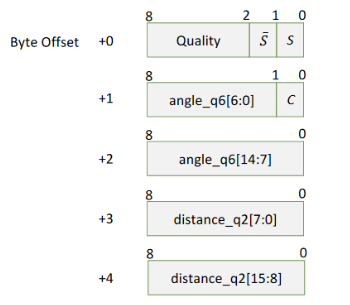
\includegraphics[width=.6\linewidth]{SYNTHESIS/protocolbreakdown.png}
			\caption{Protocol Breakdown}
			\label{fig:protocolbreakdown}
		\end{figure}
	
		So, for example, the first 6 bits of the first returned byte is used to store the scan's quality value. The idea behind the initial map processing software was to start at the beginning of the file containing binary scan data, then iterate through it by taking chunks of bits and storing them in variables.
		
		\begin{lstlisting}
		# Read in the bits according to the LIDAR response structure
		quality = f.read(6)
		inverseStart = f.read(1)
		start = f.read(1)
		angle_first = f.read(7)
		checkbit = f.read(1)
		angle_second = f.read(8)
		distance = f.read(16)
		\end{lstlisting}
		One small additional tweak that needed to be made was joining the first and second angle chunks together to form the full value.
		
		\begin{lstlisting}
		# Append the angle_q6 bits
		angle = (b"".join([angle_first, angle_second]))
		\end{lstlisting}
		
		The protocol documentation states that these aren't the true values however. The actual angle value is the binary value divided by 64 degrees, and the actual distance value is the binary value divided by 4 millimeters.
		
		\begin{lstlisting}
		# Turn binary into decimal
		# 'Actual heading = angle_q6/64.0 Degree'
		angle = (int(angle, 2) / 64.0)
		# 'Actual Distance = distance_q2/4.0 mm'
		distance = (int(distance, 2) / 4.0)/100
		\end{lstlisting}
		These points were then turned into mappable X and Y values. Despite all of this, none of this worked as intended. The produced maps made no logical sense, fig \ref{fig:failedmap} shows a map produced via this method from scans obtained from the inside of a rectangular box.
		\begin{figure}[ht]
			\centering
			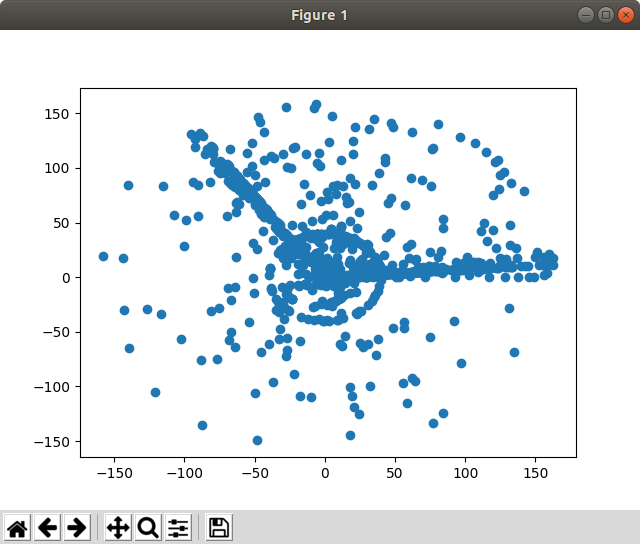
\includegraphics[width=.6\linewidth]{SYNTHESIS/failedmap.png}
			\caption{Resulting map of a box}
			\label{fig:failedmap}
		\end{figure}
	
		The generated values were printed, and it was observed that every now and then angles would be impossible values above 360. After all of this it was decided to go back to the drawing board and attempt to get the SDK working again since using the protocol was rapidly leading nowhere and burning time. Searching around on the mbed website stumbled across a robotic program that made use of a similar LIDAR system by SLAMTEC. The SDK in use there was a modified version that seemed to work fine with embedded systems, but still had all the necessary open licensing. This SDK was tested with the program and compiled fine, and is what was used to ultimately implement the robot's observational capability.
		
		\section{Memory Problems}
		It was previously assumed during the design and following some preliminary investigation into the available microcontrollers that the FRDM-K64F would be capable of storing the LIDAR readings in a temporary buffer before they are written to the file. To store the readings a two dimensional array was used, with each array entry containing a small array of two floats. To start off with the buffer used had a length of 16000, with each entry in itself containing an array of two floats (an angle and a distance). For the first few preliminary program tests this seemed to work fine, loops were used to write dummy entries to the array and the array was then written to a file to prove the process. During one test run however, a problem was shown in console along with a blinking red light on the mbed board indicating a runtime error.
		
		\begin{figure}[ht]
			\centering
			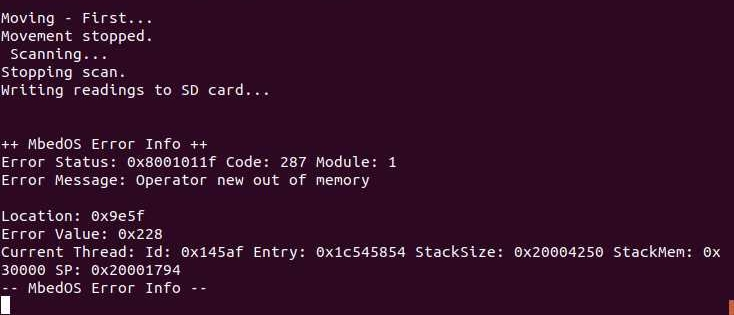
\includegraphics[width=.8\linewidth]{SYNTHESIS/memoryerror.jpg}
			\label{fig:memoryerror}
		\end{figure}
		
		This error began cropping up at the point where the program writes the buffer to a physical file. Despite it not being during the time when the readings buffer was actually filled out, the immediate reaction to the issue was simply to scale down the buffer. It made sense that perhaps too much space was being taken up by such a large variable, so it was halved to contain just 8000 angle distance pairs. The error was still encountered when compiling however, so just to see what would happen the array was decreased down to a significantly smaller size of just 1000. This issue still happened though, despite attempts to recompile and reflash the microcontroller as well as resetting the board with the reset button.
		
		\section{Scanning Inconsistency}
		One problem that repeatedly impeded development was the inconsistency in the LIDAR's scanning behaviour. Once development began to focus on writing real observational data into a buffer rather than filling it with dummy data just to prove the process, a number of issues began to crop up.
		
		The first was that occasionally entire batches of scan data would be zeroes. Every single angle and distance measurement would be a 0.0000000 float, with no changes to the buffer size making a difference. Pin connections were double checked and sometimes simply removed and plugged in again but then the scan straight after would result in the same thing happening. The troubleshooting section of the RPLIDAR A1M8 documentation was consulted. One suggestion was that the LIDAR core worked better once it had warmed up, and that it should be left spinning for a minute or so before it begins taking measurements. A simple task delay was introduced for 2 minutes before the main program loop began, but this issue would still come up sometimes. The quickest fix was generally to just recompile the program, and the issue would more often than not seemingly go away.
		
		
		
		
		